\documentclass[xelatex,13pt]{beamer}
\usetheme{metropolis}
\usefonttheme{professionalfonts} % using non standard fonts for beamer
\usefonttheme{serif}
\usepackage{helvet}
\usepackage[english]{babel}
\usepackage{graphicx}
\usepackage{textpos}
\usepackage{xcolor}
\definecolor{mauve}{rgb}{0.86, 0.82, 1.0}
\usepackage{pgfpages}
\usepackage{listings}

\lstdefinelanguage{d}{
	morekeywords={abstract,alias,align,asm,assert,auto,body,bool,break,byte,
		case,cast,catch,cdouble,cent,cfloat,char,class,const,continue,creal,
		dchar,debug,default,delegate,delete,deprecated,do,double,else,enum,
		export,extern,false,final,finally,float,for,foreach,foreach_reverse,
		function,goto,idouble,if,ifloat,immutable,import,in,inout,int,
		interface,invariant,ireal,is,lazy,long,macro,mixin,module,new,nothrow,
		null,out,override,package,pragma,private,protected,public,pure,real,
		ref,return,scope,shared,short,static,struct,string,wstring,dstring,
		super,switch,synchronized,template,this,throw,true,try,typedef,typeid,
		typeof,ubyte,ucent,uint,ulong,union,unittest,ushort,version,void,
		volatile,wchar,while,with,size_t,hash_t
	},
	sensitive=True,
	morecomment=[l]{//},
	morecomment=[s]{/\*}{\*/},
	morestring=[b]"
}

\lstset{
	language=d,
	basicstyle=\footnotesize\ttfamily, % Standardschrift
	numbers=left,               % Ort der Zeilennummern
	numberstyle=\tiny,          % Stil der Zeilennummern
	%stepnumber=2,               % Abstand zwischen den Zeilennummern
	%captionpos=b,
	numbersep=5pt,              % Abstand der Nummern zum Text
	tabsize=4,                  % Groesse von Tabs
	extendedchars=true,         %
	breaklines=true,            % Zeilen werden Umgebrochen
	showspaces=false,           % Leerzeichen anzeigen ?
	showtabs=false,             % Tabs anzeigen ?
	%frame=b,
	rulecolor=\color[cmyk]{0.0, 0.0, 0.0, 0.316},
	xleftmargin=17pt,
	%xleftmargin=0pt,
	framexleftmargin=17pt,
	framexrightmargin=5pt,
	framexbottommargin=4pt,
	keywordstyle=\color{blue},          % keyword style
	commentstyle=\color{dkgreen},       % comment style
	stringstyle=\color{red},         % string literal style
	showstringspaces=false,    % Leerzeichen in Strings anzeigen ?        
	escapeinside={/+}{+/},
	title=\lstname
}

%\setbeamertemplate{note page}{\pagecolor{yellow!5}\insertnote}\usepackage{palatino}
%\setbeameroption{show notes on second screen}

\beamertemplatenavigationsymbolsempty

\usepackage{xkeyval}
%\presetkeys{todonotes}{inline}{}
\usepackage[disable]{todonotes}

\title{Asynchronous single page applications without a line of HTML or
Javascript.}
\subtitle{Or why D is just awesome}
\author{Robert "burner" Schadek}
\date{May 5, 2016}
\institute{DConf}

\begin{document}
\maketitle

\begin{frame}
	\frametitle{Javascript and HTML are \textbf{awesome}}
	\begin{itemize}
		\item No explicit types
		\item Variables may be undefined
		\item Repetition repetition repetition
		\item No templates
		\item No compile time function execution
			\pause
		\item No compile time
	\end{itemize}
	\note[item]{Very quickly go through the points and stop for dramatic pause}
\end{frame}


\begin{frame}[plain]
\begin{textblock*}{0cm}(-1cm,-4.2cm)
	
\includegraphics[width=1.0\paperwidth]{picardriker.jpg}
\end{textblock*}
	\note[item]{I know what you are thinking.}
	\note[item]{Walter, Andrei and the other screwed up letting me present
	here.}
\end{frame}

\begin{frame}
	\frametitle{Goals}	
	\begin{itemize}
		\item Retain type-information of data from DB to Client's Browser
			\pause
		\item Keeping things DRY	
			\pause
		\item Get things done
	\end{itemize}
\end{frame}

\section{Vibe.d and Diet}
\begin{frame}
	\frametitle{Vibe.d}
	\begin{itemize}
		\item Powerful asynchronous I/O and web toolkit for D
			\pause
		\item uses Fibers and Threads
			\pause
			\begin{itemize}
				\item \(n \rightarrow m\) mapping
					\pause
				\item \lstinline@yield()@
					\pause
				\item async io
			\end{itemize}
			\pause
		\item async DB connectivity for MongoDB, Redis, MySQL
			\pause
		\item Rest interface generator
			\pause
		\item Web interface generator
			\pause
		\item Diet
	\end{itemize}
\end{frame}

\section{Typescript and AngularJS}
\begin{frame}
	\frametitle{Typescript and AngularJS}
\end{frame}

\section{Dataflow from the Frontend to the Database and back again}
\begin{frame}
	\frametitle{Dataflow from the Frontend to the Database and back again}
\end{frame}

\section{Testing and Debugging}
\begin{frame}
	\frametitle{Testing and Debugging}
	\note[item]{Of course we are perfect programmers and never make mistakes,
	\textbf{BUT}.}
\end{frame}

\section{Everything is wrong}
\begin{frame}
\begin{textblock*}{0cm}(-1cm,-4.2cm)
	
\includegraphics[width=1.0\paperwidth]{picarddday.jpg}
\end{textblock*}
\end{frame}

\begin{frame}
	\frametitle{Everything is wrong}
	\begin{itemize}
		\item all we solved was a tiny specific problem
		\item what about server to database
		\item what if we would use Dart instead of Typescript
		\item how do we communicate the overall architecture
		\item how do we keep the architecture in sync with the code
		\item how do we communicate with non-developer
		\item ...
		\pause
		\item {\huge How do we deal with change?}
	\end{itemize}
\end{frame}

\begin{frame}
	\frametitle{Everything is still wrong}
	\begin{itemize}
		\onslide<1->{\item Waterfall Model} \onslide<2->{\(\leftarrow\) no change, never}
		\onslide<7->{\item UML} \onslide<8->{\(\leftarrow\) just kill me
			already}

		\item[] { \onslide<1-8>{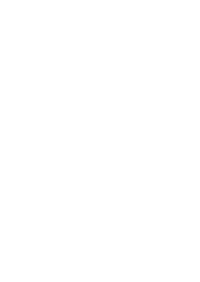
\includegraphics[width=0.3\textwidth]{Stick1.png}}
				\only<9>{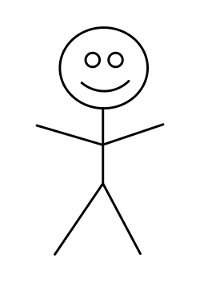
\includegraphics[width=0.3\textwidth]{Stick.png}}
				\only<10>{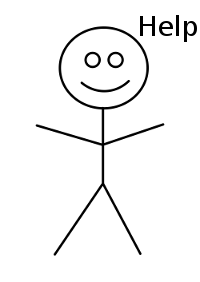
\includegraphics[width=0.3\textwidth]{Stick2.png}}
		}

		\onslide<5->{\item agile Methods} \onslide<6->{\(\leftarrow\) just
			hacking, with fancy names}
		\onslide<3->{\item just Hacking} \onslide<4->{\(\leftarrow\) no plan
			to speak of, just change}
		
	\end{itemize}
	
\end{frame}

\begin{frame}
	\frametitle{What do we want}
	\begin{itemize}
		\item speak about the system at different levels of detail\\
		with different people
		\item quickly introduce people to the system
		\item keep data classes (Model) synchronized across
		\begin{itemize}
			\item Frontend
			\item Server
			\item Database
		\end{itemize}
		\item write only one model for everything, to keep stuff in sync
		\item have description line based, because git
		\item generate everything possible from the
	\end{itemize}
\end{frame}

\section{Introducing C4 Architecture}
\begin{frame}[plain]
\begin{textblock*}{0cm}(-1cm,-4.7cm)
	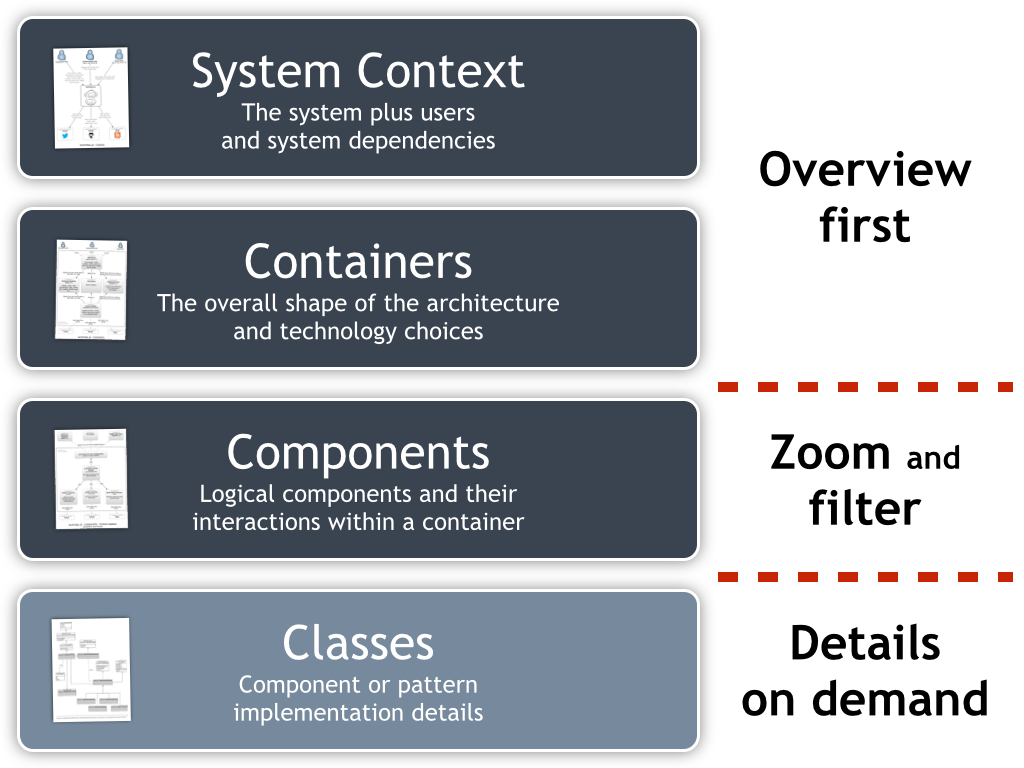
\includegraphics[width=1.0\paperwidth]{c4overview.png}
\end{textblock*}
\end{frame}
\begin{frame}[plain]
\begin{textblock*}{0cm}(-1cm,-4.7cm)
	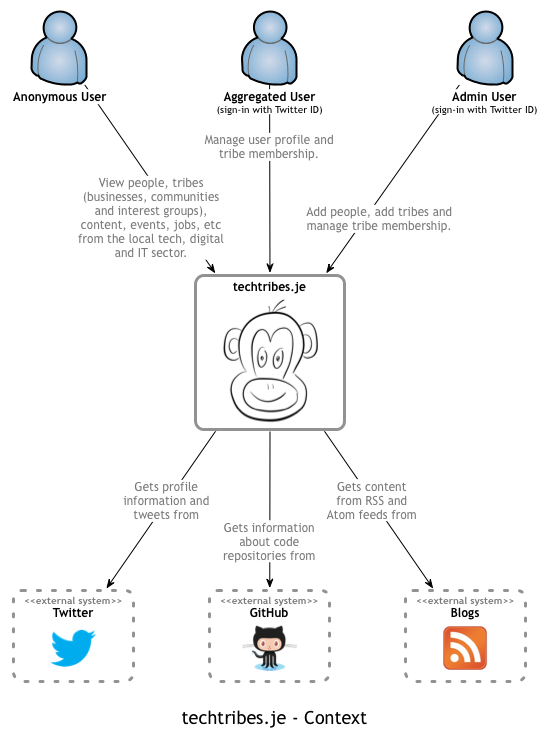
\includegraphics[width=1.0\paperwidth]{c4systemcontext.png}
\end{textblock*}
\end{frame}
\begin{frame}[plain]
\begin{textblock*}{0cm}(-1cm,-11.7cm)
	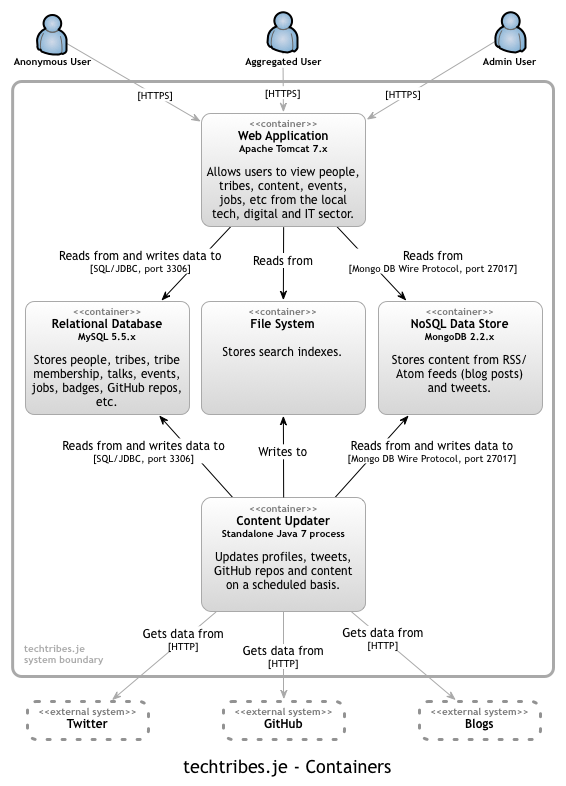
\includegraphics[width=1.0\paperwidth]{c4container.png}
\end{textblock*}
\end{frame}
\begin{frame}[plain]
\begin{textblock*}{0cm}(-1cm,-4.7cm)
	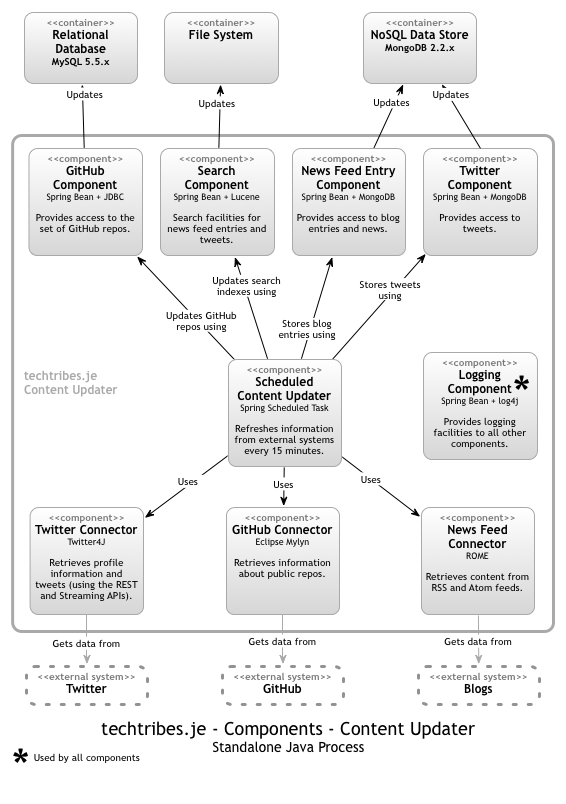
\includegraphics[width=1.0\paperwidth]{c4components.png}
\end{textblock*}
\end{frame}

\begin{frame}
	\frametitle{C4 Architecture Structurizer}
	\begin{itemize}
		\item Implements C4 Architecture Model 
		\item Java Library with classes to build this model
		\begin{itemize}
			\item its code, its fits into git
		\end{itemize}
		\item Structurizer generates code
		\item {\huge only Java spring and .net}
	\end{itemize}
\end{frame}
\begin{frame}[plain]
\begin{textblock*}{0cm}(-1cm,-4.2cm)
	
\includegraphics[width=1.0\paperwidth]{picardwtf.jpg}
\end{textblock*}
\end{frame}

\section{How hard can it be}
\begin{frame}
	\frametitle{How do we approach the development}
	\begin{itemize}
		\item we're not gone create a new language\pause, at first\pause,
			most likely
		\item the model (ast) is pretty simple
		\begin{itemize}
			\item the world has
			\item actors, software/hardware systems
			\item a software systems has
			\item containers (everything with a unique pid)
			\item a container has
			\item components (think \lstinline@module@) and classes
			\item a component has
			\item components and classes
			\item[]
			\item connections between the above
			\begin{itemize}
				\item UML Association, Aggregation, Composition, Dependency
			\end{itemize}
			\item additional informations, names, descriptions
		\end{itemize}
	\end{itemize}
\end{frame}

\begin{frame}[fragile]
	\frametitle{How do we continue}
	\begin{itemize}
		\item we can add a single class to multiple containers and components
		\item a class has member variable and member functions
		\item Types \pause e.g. strings are not always string
		\begin{itemize}
			\item D string
			\item MySQL text
			\item C++ std::string
		\end{itemize}
	\end{itemize}
\end{frame}
\begin{frame}[fragile]
	\frametitle{The Type Problem Solution}
\begin{lstlisting}
struct Type {
    string name;
    string[string] typeMapping;
}

Type passwordHash;
str.name = "PasswordString";
str.typeMappings["D"] = "string";
str.typeMappings["MySQL"] = "VARCHAR(128)";
\end{lstlisting}
\pause
\begin{itemize}
	\item key \(=\) container name
	\item value \(=\) name of type as used by the language of the container
\end{itemize}
\end{frame}

\section{Miscellaneous}
\begin{frame}
	\frametitle{Miscellaneous}
	\todo{GC Angst}
	\todo{Deployment}
	\todo{Performance Tuning}
	\todo{HTTPS}
\end{frame}

\begin{frame}[plain]
\begin{textblock*}{0cm}(-1cm,-4.2cm)
	
\includegraphics[width=1.0\paperwidth]{picardpuppy.png}
	\todo{http://gryphon-shifter.deviantart.com/art/Captain-Picard-and-Puppies-458352865}
\end{textblock*}
\end{frame}

\end{document}
